% context: 9th-grade physics classwork, in-class review for the Unit 1 measurement quiz
% topic: significant figures, rounding, scientific notation, reading a ruler,
%        unit conversion, average speed
% structure: two pages of deliberately easy problems, widely spaced for written work
\documentclass[12pt, twoside]{article}
\input{../preamble}
\usepackage{float}

\title{Physics}
\author{Chris Huson}
\date{September 2026}

\fancyhead[LE]{\thepage}
\fancyhead[RO]{\thepage \\ Nickname: \hspace{2.25cm} \,\\ \,}
\fancyhead[LO]{La Scuola d'Italia / Huson / Physics \\* 24 September 2026}

\begin{document}

\subsubsection*{1.4 Classwork: Measurement quiz review}

\textbf{Reference (provided).} \quad
average speed $= \dfrac{\text{distance}}{\text{time}}$ \\[0.1cm]
1 in. = 2.54 cm \quad 1 m $\approx$ 3.28 ft \quad 1 km = 1000 m \\
1 m = 100 cm \quad 1 cm = 10 mm \quad 1 h = 3600 s

\vspace{0.3cm}

\begin{enumerate}[itemsep=0.6cm]

\item Write down the number of significant digits in each measurement.
  \begin{multicols}{3}
    \begin{enumerate}[itemsep=0.5cm]
      \item 7.25 m
      \item 3.0 s
      \item 0.045 kg
      \item 105 g
      \item 20.10 cm
      \item $6.0 \times 10^{3}$ m
    \end{enumerate}
  \end{multicols} \vspace{0.6cm}

\item Round each value to three significant figures. Copy the calculator display
  followed by three dots, then round: $\sqrt{2} = 1.4142135\ldots \approx 1.41$
  \begin{multicols}{2}
    \begin{enumerate}[itemsep=1.5cm]
      \item $\sqrt{10}$
      \item $\dfrac{1}{7}$
    \end{enumerate}
  \end{multicols} \vspace{1.3cm}

\item Write in scientific notation, rounded to three significant figures.
  \begin{multicols}{2}
    \raggedright
    \begin{enumerate}[itemsep=1.5cm]
      \item The distance from the Earth to the Sun, 149{,}600{,}000 km
      \item The thickness of a sheet of paper, 0.000102 m
    \end{enumerate}
  \end{multicols} \vspace{1.3cm}

\item Write each value as an ordinary decimal number.
  \begin{multicols}{2}
    \raggedright
    \begin{enumerate}[itemsep=1.5cm]
      \item The height of Mount Everest, $8.849 \times 10^{3}$ m
      \item The mass of a paper clip, $1.0 \times 10^{-3}$ kg
    \end{enumerate}
  \end{multicols}

\newpage

\item The bar below is measured with a centimeter ruler marked in millimeters.

\begin{center}
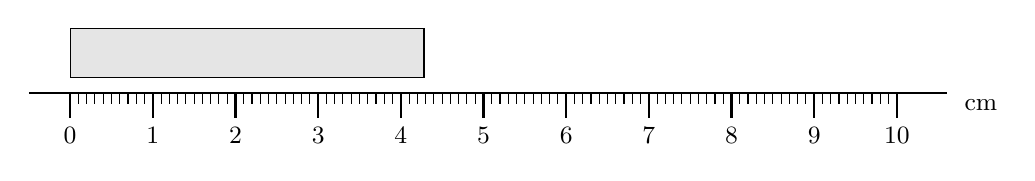
\begin{tikzpicture}[scale=1.05]
  \draw[fill=gray!20] (0,0.18) rectangle (4.28,0.78);
  \draw[thick] (-0.5,0) -- (10.6,0);
  \foreach \x in {0.1,0.2,...,9.95}{\draw (\x,0) -- (\x,-0.14);}
  \foreach \x in {0,1,2,3,4,5,6,7,8,9,10}{\draw[thick] (\x,0) -- (\x,-0.3) node[below] {\small \x};}
  \node[right] at (10.7,-0.15) {\small cm};
\end{tikzpicture}
\end{center}

  \begin{enumerate}[itemsep=0.9cm]
    \item Record the length of the bar. Include one estimated digit --- the last
      digit, the one you are not certain of.
    \item Write the same length in millimeters, and again in meters.
  \end{enumerate} \vspace{0.9cm}

\item Convert between units, rounding to three significant figures. Write the
  conversion as a fraction and show the units cancelling.
  \begin{enumerate}[itemsep=2.0cm]
    \item The Leaning Tower of Pisa is 56.7 meters tall. What is its height in feet?
    \item A sheet of US letter paper is 11.0 inches long. What is its length in
      centimeters?
  \end{enumerate} \vspace{1.8cm}

\item A student walks 60.0 meters down the hallway in 45.0 seconds. Find the
  average speed in meters per second, rounded to three significant figures.
  \vspace{2.0cm}

\item A Category 1 hurricane has winds of at least 119 kilometers per hour. What is
  this speed in meters per second? Write the conversion as a single chain of
  fractions.

\end{enumerate}
\end{document}
